\documentclass[12pt,compress]{beamer}
\usepackage{ifthen,verbatim}

\title{Moving Muon Chambers \\ in an Alignment Module}
\author{Jim Pivarski}
\institute{Texas A\&M University}
\date{20 October, 2006}

\setbeamertemplate{navigation symbols}{}
\setbeamertemplate{headline}{\includegraphics[height=1 cm]{../cmslogo} \hspace{0.1 cm} \includegraphics[height=1 cm]{../tamulogo} \hfill
\begin{minipage}{9 cm}
\vspace{-0.75 cm} \small
\begin{center}
\ifthenelse{\equal{\insertpagenumber}{1}}{}{\insertsection}
\end{center}
\end{minipage} \hfill
\begin{minipage}{1 cm}
\vspace{-0.75 cm} \small
\begin{center}
\ifthenelse{\equal{\insertpagenumber}{1}}{}{\insertpagenumber/\pageref{numpages}}
\end{center}
\end{minipage}}

\xdefinecolor{verylightgray}{rgb}{0.95,0.95,0.95}
\beamertemplateshadingbackground{verylightgray}{white}

\begin{document}
\frame{\titlepage}
\section*{Muon Alignment Module --- Jim Pivarski}

\begin{frame}
\frametitle{Two Topics}
\begin{enumerate}\setlength{\itemsep}{1 cm}
\item Verifying Andre's tools
\item New Analyzer-based Framework for Alignment
\end{enumerate}
\vfill
\end{frame}

\begin{frame}
\frametitle{Andre's Tools: Checklist}

Test: can I move global hit positions?

\begin{enumerate}[$\surd$ ]\setlength{\itemsep}{0.5 cm}
\item \textcolor{blue}{Read geometry from a remote database} \\ (PoolDBESSource with connect = "frontier: \ldots")
\item \textcolor{blue}{Create a local file with randomly-generated misalignments} \\ (MisalignedMuonESProducer and PoolDBOutputService)
\item \textcolor{blue}{Read geometry from local file} \\ (PoolDBESSource with connect = "sqlite\_file: \ldots")
\item \textcolor{blue}{Create a local file with user-controlled geometry} \\ (MuonAlignment class with PoolDBOutputService)
\end{enumerate}
\end{frame}

\begin{frame}
\frametitle{Proof that it Works}
\begin{center}
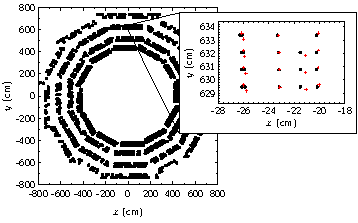
\includegraphics[width=0.9\linewidth]{misalignment_producer}

$\bullet$ is ideal, \textcolor{red}{$+$ is misaligned ("ShortTermScenario")}
\end{center}
\end{frame}

\begin{frame}
\frametitle{New Muon Alignment Analyzer}

\textcolor{blue}{MuonAlignmentAnalyzer} reads an alignment, computes corrections, and writes a new alignment

\vfill
\begin{description}
\item[maa\_iteration0.cfg]
\end{description}
\vspace{-0.5 cm}
\begin{center}
MisalignedMuonESProducer $\to$ {\tt maa\_iteration0.db}
\end{center}

\begin{description}
\item[maa\_iteration1.cfg]
\end{description}
\vspace{-0.5 cm}
\begin{center}
MuonAlignmentAnalyzer $+$ data $\to$ {\tt maa\_iteration1.db}
\end{center}

\begin{description}
\item[maa\_iteration2.cfg]
\end{description}
\vspace{-0.5 cm}
\begin{center}
MuonAlignmentAnalyzer $+$ data $\to$ {\tt maa\_iteration2.db}
\end{center}
\end{frame}

\begin{frame}[fragile]
\frametitle{Structure of MuonAlignmentAnalyzer}
\begin{description}
\item[Generalized: Not Limited to One Algorithm]
\end{description}
\hspace{1 cm} \begin{minipage}{\linewidth}
\scriptsize
\begin{verbatim}
module analyzer = MuonAlignmentAnalyzer
{
    string algo = "dummy"

    string output = "maa_iteration1.root"
    string src = "globalMuons"
    uint32 events = 900
}
\end{verbatim}
\end{minipage}

\vfill
\begin{itemize}\setlength{\itemsep}{0.25 cm}
\item MuonAlignmentAnalyzer points to a \textcolor{blue}{MuonAlignmentAlgo}
\item Sub-class \textcolor{blue}{MuonAlignmentAlgoDummy} does the real work
\item algo = "dummy" $\to$ selects \textcolor{blue}{MuonAlignmentAlgoDummy}
\end{itemize}
\end{frame}

\begin{frame}
\frametitle{Test-Drive of MuonAlignmentAnalyzer}
\begin{center}
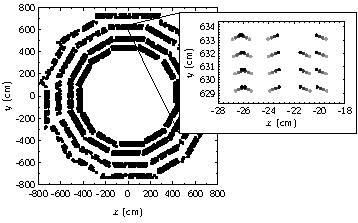
\includegraphics[width=0.85\linewidth]{misalignment_analyzer}

MuonAlignmentAlgoDummy moves every chamber with a hit $+0.25$ cm in $x$, $+0.10$ cm in $z$ (4 iterations)
\end{center}
\end{frame}

\begin{frame}
\frametitle{Awkward Feature}

\begin{itemize}
\item We want to call MuonAlignment.saveToDB() at the end of the job
\item but if we put this call in MuonAlignmentAnalyzer's destructor, it writes incorrectly (13k instead of 2.1MB)
\item this is presumably because the structures necessary for database-writing were deleted before my analyzer
\item For now, I stop after the 900th event and ignore the rest\ldots
\end{itemize}

\vfill
Do analyzers have a method that is called after all data-taking and before deletion?
\end{frame}

\begin{frame}
\frametitle{Future Plans}
\begin{enumerate}\setlength{\itemsep}{0.4 cm}
\item Calculate track$-$hit residuals
\begin{itemize}
\item talk to Jean-Roch Vlimant (UCSB)
\item and Francisco Matorras (Santander)
\end{itemize}

\item Dead-reckon alignment from trends in residuals plots (MuonAlignmentAlgoResiduals)
\begin{itemize}
\item e.g.\ offset in $x$ residual $\Rightarrow$ move $x$
\item linear trend in $y$ residual $\Rightarrow$ rotate $\phi_z$
\end{itemize}

\item Incorporate Santander group's algorithm (MuonAlignmentAlgoMillipede)

\item Incorporate HIP, Kalman, CMS NOTE 2006/016\ldots
\end{enumerate}
\end{frame}

\begin{frame}
\frametitle{Summary}
\begin{itemize}\setlength{\itemsep}{1 cm}
\item Thank you Andre! (and Fr\'ed\'eric!)
\item We have a generalized framework for Muon Alignment
\end{itemize}
\label{numpages}
\end{frame}

\begin{frame}
\frametitle{Extra slide: Surprises (to me)}

\begin{tabular}{p{0.07\linewidth} p{0.9\linewidth}}
  \begin{minipage}{\linewidth}
    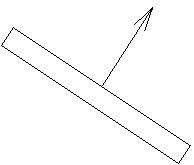
\includegraphics[width=\linewidth]{local_coordinates}
  \end{minipage} &
  \begin{minipage}{\linewidth}
    direction away from IP is $z$ in local coordinates, not $y$
  \end{minipage}
\end{tabular}

\vfill
$+z$ is toward the IP for some chambers, away for others

\vfill
Wire DetIds $\neq$ detector DetIds
\begin{itemize}
\item need to recursively search detector for wire
\item I made a map$<$long,long$>$ to quickly match wire to detector
\end{itemize}
\end{frame}

\end{document}
